\documentclass[10pt]{amsart}

\usepackage{color}
\usepackage{enumitem}
\usepackage{verbatim}
\usepackage{graphicx} 
\usepackage{fancyhdr}

\setlength{\headsep}{.33in}
\setlength{\topsep}{0in}
\setlength{\topmargin}{-1in}
\setlength{\topskip}{0in}    % between header and text
\setlength{\textheight}{10in} % height of main text
\setlength{\textwidth}{7.05in}    % width of text
\setlength{\oddsidemargin}{-0.30in} % odd page left margin
\setlength{\evensidemargin}{-0.30in} % even page left margin
\setlength{\parindent}{0in}   % remove paragraph indenting

\linespread{1.13}

\newcommand{\head}[1]{
   \begin{tabular*}{7.1in}{@{}l@{\extracolsep{\fill}}r}
      Russell Frank & \today \\
   \end{tabular*}
   \begin{center} \LARGE #1 \normalsize \end{center}
   \vskip 0.1in
}

\def\wl{\par \vspace{\baselineskip}}

\pagestyle{fancy}
\fancyhead[R]{rfranknj \thepage / 4}

\begin{document}

\head{Data Science HW 1}

\begin{tabular}{l|l}
  1a & 2 \\
  1b & 2 \\
  1c & 2 \\
  1d & 2 \\
  1e & 2 \\
  1f & 2 \\
  1h & 3 \\
  1i & 3 \\
  2 & 3 \\
  3 & 3 \\
  4 & 4 \\
  5 & 4 \\
  6 & 4 \\
  7 & 4 \\
\end{tabular}

\newpage

\textbf{1a.}

\begin{tabular}{ll}
  producer & nominal \\
  release\_to\_review\_time & interval \\
  rating & ordinal \\
  helpfulness & ratio \\
  number\_of\_votes & ratio \\
  length\_of\_review\_text & ratio \\
\end{tabular}

\textbf{1b.} Apple. \\

\textbf{1c.} 52.9681794471 \\

\textbf{1d.} 52.9681794471 \\

\textbf{1e.} 

\begin{tabular}{ll}
  min & -537 \\
  Q1 & 75.0 \\
  median & 144 \\
  Q3 & 290.0 \\
  max & 11686 \\
\end{tabular}

\wl

The interquartile ranges are 215. \\

A box and whisker plot is a nice way to show quartiles.\\

\textbf{1f.} \\

\fbox{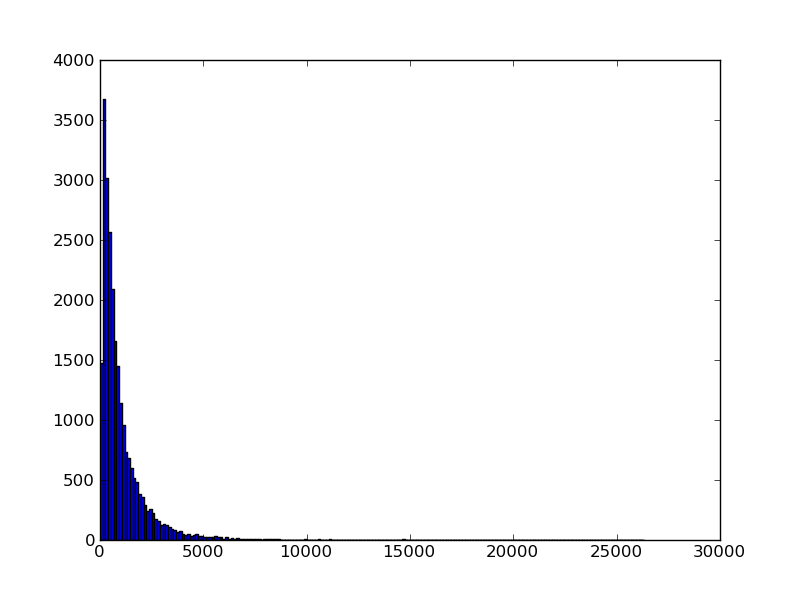
\includegraphics[width=6in]{length_plot.png}}

\textbf{1g.} Yes, it is obviously skewed, looking at the histogram.

`Sony', `1516', `0', `0', `5', `0.96', `25', `26332' \\
`Asus', `101', `0', `1', `5', `0.945', `128', `22492' \\
`Lenovo', `231', `0', `0', `3', `0.853', `34', `18275' \\

\textbf{1h.} 0.25054940649068008 \\

So, there is a correlation between the length of reviews and their helpfullness.
In general, lengthier reviews are more helpful. Shorter reviews don't have
enough information to be helpful. 

\textbf{1i.} \\

\fbox{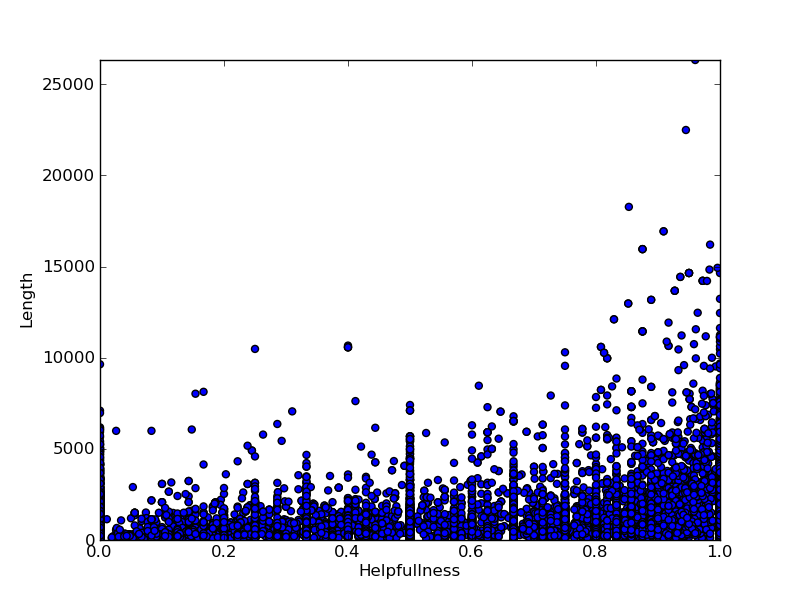
\includegraphics[width=6in]{length_helpfullness_scatter.png}}

\textbf{2.} \\
  $w = 0.216, x = 0.064$ \\
  $y = 0.84, z = 0.64$ \\

  We went over the theorems regarding AND and OR constructions for families of
  hash functions in class. \\

\textbf{3a.} \\

  $u = [1, -1, 1]$ \\ 
  $v = [1, -1, 1]$ \\ 
  $w = [-1, 1, 1]$ \\

  Basically, each bit in the sketch is 1 if the dot product between the
  vector in question and the hyperplane is $> 0$ and -1 if the dot product 
  is $< 0$. \\

\textbf{3b.} \\

Similarity sketch(u) sketch(v): 1.0 \\
Similarity sketch(u) sketch(w): -0.333333333333 \\

\textbf{4a.} 

The Mahalanobis distance reduces to the Euclidean distance when the covariance
matrix is the identity. This is the case when the covariance is 0 between each
different random variable, and obviously the ones on the diagonal correspond to
the covariance between a random variable and itself, which is 1. \\

\textbf{4b.} 

When the covariance matrix is a diagonal matrix, the Mahalanobis distance
reduces to the normalized Euclidean distance. In this case, we have random
variables which have some differing variance; and the normalized Euclidean
distance is exactly what it sounds like: a normalized distance. The inverse
of this diagonal matrix is therefore going to be $\frac{1}{\delta}$, where
$\delta$ is the variance of the corresponding variable. Since it's in the
denominator, it ends up dividing each component of the distance, resulting in
a normalized distance. \\

\textbf{5a.} \\

Signature of document 1 : 5 2 0 \\
Signature of document 2 : 1 2 1  \\
Signature of document 3 : 1 2 4 \\
Signature of document 4 : 1 2 0 \\

\textbf{5b.} Only the last function is a true permutation. \\

\textbf{5c.} \\

s 1 and s 2 estimation 0.333333333333 actual 0.0 \\
s 1 and s 3 estimation 0.333333333333 actual 0.0 \\
s 1 and s 4 estimation 0.666666666667 actual 0.25 \\
s 2 and s 3 estimation 0.666666666667 actual 0.0  \\
s 2 and s 4 estimation 0.666666666667 actual 0.25 \\
s 3 and s 4 estimation 0.666666666667 actual 0.25 \\

\textbf{6.} \\

\begin{tabular}{l}
  \textbf{A} \\

  % Mr. and Mrs. Dursley of number four, Privet Drive, were proud to say that they 
  % were perfectly normal, thank you very much.

  and Mrs. Dursely \\
  of number four\\
  to say that \\
  that they were \\

\end{tabular}

\begin{tabular}{l}
  \textbf{B} \\

  % Not for the first time, an argument had broken out over breakfast at number four, 
  % Privet Drive.

  for the first \\
  the first time \\
  an argument had \\
  at number four \\

\end{tabular}

\wl

The jaccard similarity is 0. There is no intersection of the shingles. \\

\textbf{7.} The logit function transforms values in the range 0 to 1 to the
entire real line.

\end{document}
